\section{Introduction}
\label{sec:Introduction}

Robots are becoming increasingly important, targeting human assistance at home or at the workplace. Yet, such robots can not be pre-programmed to face every day problems in our open ended and dynamic environments. This challenge requires to develop learning algorithm for the robot to adapt to its environment. Among other forms of adaptation to the environment, \textit{social learning}, where knowledge is transmitted from humans to robots through social interaction, is of primordial importance. It has the advantage of being an intuitive way for humans to instruct robots. A usual assumption in such systems is that the learner and the teacher share a mutual understanding of the meaning of each others' signals, and in particular the robot is usually assumed to know how to interpret teaching instructions from the human. In practice, the range of accepted instructions is limited to the one predifined by the system developer. However non-expert users might have very different preferences and predefined instructions might not be well accepted. We believe that robots should themselves be able to adapt progressively to every user's particular teaching behaviors at the same time as they learn new skills. %The aim of this work is to make a first step in this direction.
%in order for a robot to learn from a human user, it must be possible for humans to communicate their intentions and preferences to such machines. 

Research in robotics has long been inspired by human social learning. Among other aspects, learning by demonstration/imitation has attracted most attention. It has provided several examples of efficient learning in robotic systems \cite{Argall09lfdsurvey}\cite{lopes10imitationchapter}. Data from a human teacher has been used as initial condition for further self-exploration in robotics \cite{nicolescu2003natural}, bootstrapping further intrinsically motivated learning \cite{nguyen2011bootstrapping}, information about the task solution \cite{Calinon07}, information about the task representation \cite{macl07affimit}, among others. Several representations have been used to generalize the demonstration data using reinforcement learning \cite{Thomaz2008}, inverse reinforcement learning \cite{macl07affimit}\cite{Abbeel04icml}, or regression methods \cite{Calinon07}\cite{chernova09jair}. The different formalisms make use of various kinds of information and extract different knowledge, either direct policy information or a reward function that explains the behavior.
%
\begin{figure}[!t]
	\begin{center}
   		%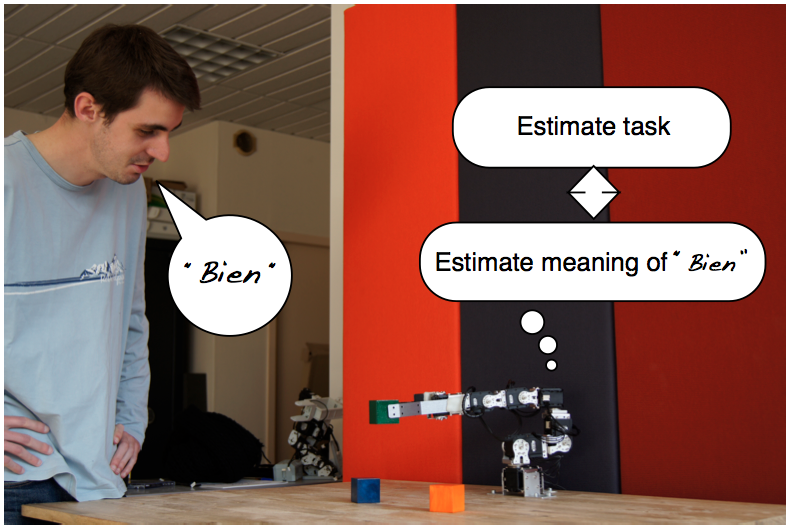
\includegraphics[width=0.8\columnwidth]{images/exp2.png}
   		%\caption{A human teacher is interacting with a robot using spoken language. The provided teaching signals allow the robot, which does not know before hand their associated meanings, to estimate simultaneously what the task is and the meaning of the spoken words.}
   		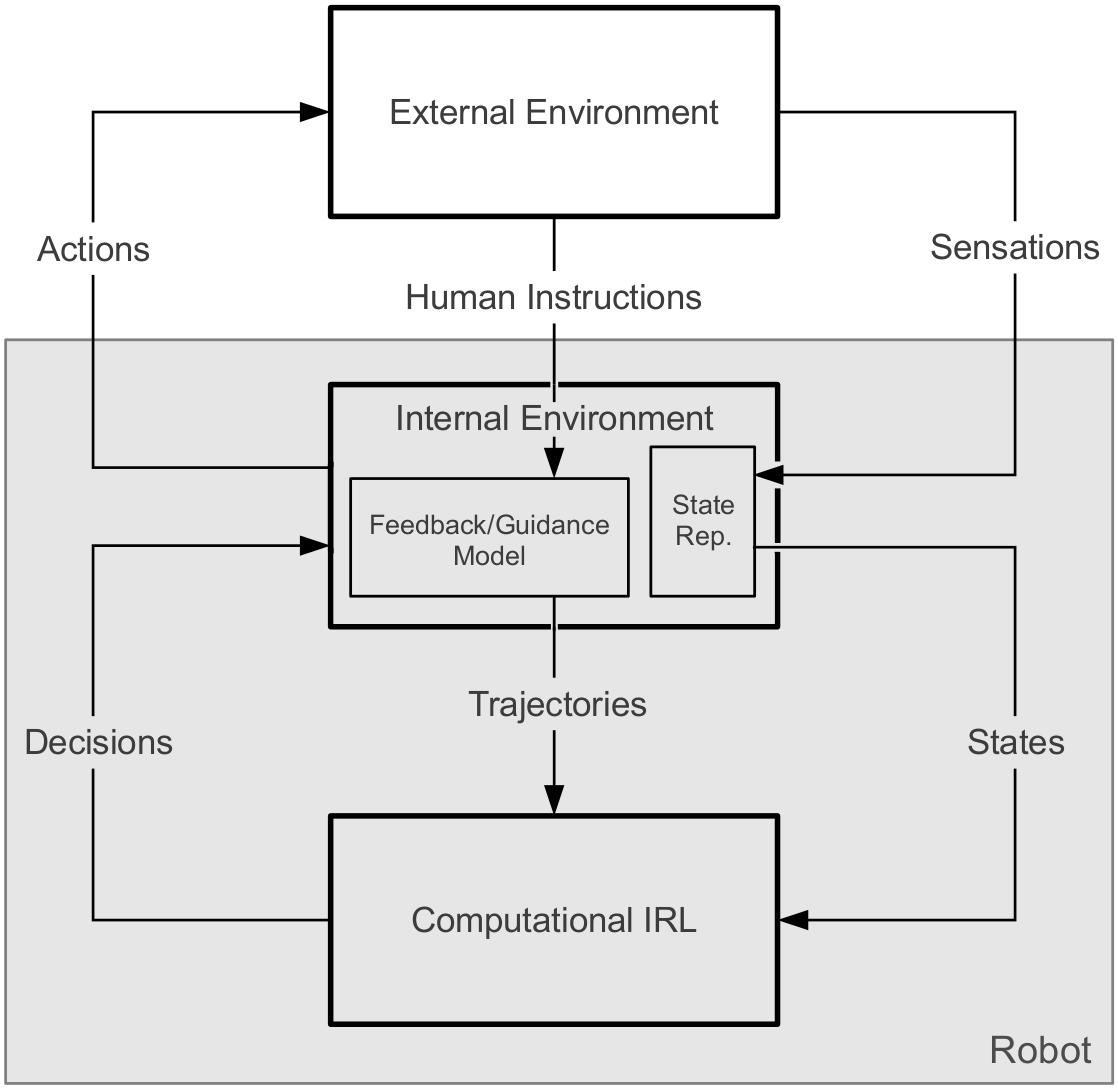
\includegraphics[width=0.8\columnwidth]{images/problem_representation.png}
   		\caption{Reinforcement learning oriented architecture of our problem. Humans provide instructions for learning a task whose meanings are a priori unknown. Thus, the meaning of these instructions has to be learnt by the robot in addition to learning the task itself.}
		\label{fig1} 
   \end{center}
\end{figure}

For most of those systems, the human demonstrations are provided in a batch perspective where data acquisition is done before the learning phase. Recently it has been suggested that \textit{interactive learning} \cite{nicolescu2003natural}\cite{Breazeal2004} might be a new perspective on robot learning, that combines the ideas of learning by demonstration, learning by exploration and tutor feedback. Under this approach the teacher interacts with the robot and provides extra feedback or guidance. In addition, the robot can act to improve its learning efficiency. Approaches have considered: extra reinforcement signals \cite{Thomaz2008}, action requests \cite{macl09airl}, disambiguation among actions \cite{chernova09jair}, preferences among states \cite{Mason2011}, iterations between practice and user feedback sessions \cite{judah2010rlandcritique}, and choosing actions that maximize the user feedback \cite{knox2009interactively}. %In \cite{Cakmak2010a} the authors compare the results when the robot has the option of asking or not the teacher for feedback, and in \cite{cakmak2012designing} study what it means for a robot learner to ask good questions.

An important challenge for such interactive systems is to deal with nonexpert humans. Several studies discuss the various behaviors naive teachers use when instructing robots \cite{Thomaz2008,Cakmak2010}. An important aspect is that the feedback is frequently ambiguous and deviates from the mathematical interpretation of a reward; or a sample trajectory deviates from an optimal policy. For instance, in the work of \cite{Thomaz2008} the teachers frequently gave a positive reward for exploratory actions even if the signal was used by the learner as a standard reward. Also, even if we can define an optimal teaching sequence, humans do not necessarily behave according to those strategies \cite{Cakmak2010}.

In addition, users may have various expectations and preferences when interacting with a robot; therefore predifined protocols or teaching signals may bother the user and dramatically decrease the performance of the learning system \cite{rouanet2013impact}. In this paper, we present an algorithm allowing a robot to learn the meaning of human teaching instructions in the process of learning a task (as illustrated in figure~\ref{fig1}). Importantly, the system does not need bootstraping with known instructions, but only requires knowledge about the possible structures of meanings and tasks. The learnt instruction-to-meaning association can then be reused in the learning of novel tasks, progressively increasing the knowledge of the robot. We will also show that, by combining known and unknown teaching signals, the robot is able to take advantages of unknown instructions to learn more efficiently than by relying only on known ones. We do not claim that we should not rely on predefined signals but rather that the feedback or guidance provided through predefined protocols could be completed with the particular teaching signals that each user provides.

We extend the work presented in \cite{macl11simul}, which introduced a preliminary approach to this problem considering an abstract symbolic space of instructions in simulation. Here, we allow the robot to learn the meaning of unknown instructions without the need of bootstrapping the system with known instructions and by considering real natural speech waves data instead of symbolic labels, as well as a physical human-robot interaction scenario. In \cite{heckmann2009teaching}, the robot ASIMO is taught to associate new spoken signals to visual object properties, both in noisy conditions and without the need for bootstrapping. However the robot is not learning a sequential task but correlations between clusters in speech and visual spaces. Similarly Kindermans et al. \cite{Kindermans2012a} proposed an unsupervised training of a P300-based BCI systems using application constraints. Their formalism is close to the one described in this paper; however, our system is able to provide a confidence about its current knowledge of the task and instruction-to-meaning association.

Our algorithm differs from typical learning by demonstration systems because data is acquired in an interactive and online setting. It improves from previous learning by interaction systems in the sense that the instructions received are continuous unlabelled signals. Our framework is generic and the signals provided by the teacher can be gestures, facial expression, or any modalities as long as we can project them into a fixed length continuous representation.

%; and that they form differentiable clusters in such space. In addition, the algorithm is able to recover from teaching mistake, i.e. when the user send an inappropriate signals to the robot (e.g. saying \textit{'Correct'} instead of \textit{'Wrong'}).

Our contribution is threefold: a) we provide an online learning algorithm which makes it possible to learn the meaning of unknown and noisy instructions, as well as a new task at the same time, b) we enable the reuse of acquired knowledge about instructions for learning new tasks, and c) in the case where the robot initially knows some of the instructions meanings, extra unknown teaching signals are used to improve learning efficiency.

In Section~\ref{sec:Algorithm}, we will provide details on the algorithm. % which is general and does not make particular assumptions on how the task or the instructions are represented. 
The following sections present an application of this algorithm to a particular interaction scenario. We will introduce first the robotic system, the interaction protocol and the signals processing unit. Finally, we will present results from both simulations and an experiment with a real robot.


%Concretely the robot can learn a task from isolated words in any languages or sounds such as hand clapping (e.g. the user could use the word \textit{``Dog''} to mean \textit{``Correct''}). In addition the user is free to teach any task (from a set of possible one) to the robot. Both task and speech signals to meanings association are learnt simultaneously, meaning that no previous user specific training are needed. However the interaction protocol is constrained to be turn taking and possible signals meanings are reduced to feedback or guidance on the robot's actions.






